% !TEX program = xelatex
\documentclass[blue,normal,cn,hide]{elegantbook}

\usepackage{pdflscape}
\usepackage{tabu}
\usepackage{booktabs} 
\usepackage{colortbl} 
\usepackage{xcolor} 
\usepackage{xfrac}
\usepackage{tikz}
\usepackage{titling}
\usepackage{bytefield}
\usepackage{longtable}
\renewcommand\maketitlehooka{\null\mbox{}\vfill}
\renewcommand\maketitlehookd{\vfill\null}

\title{Sirius 设计文档}
\version{0.01}
\date{\today}
\author{}

\makeatletter
\let\thetitle\@title
\let\theauthor\@author
\let\thedate\@date
\makeatother

\pagestyle{fancy}
\fancyhf{}
\rhead{\theauthor}
\lhead{\thetitle}
\cfoot{\thepage}

\begin{document}

\begin{titlepage}
    \vspace*{\fill}
    \begin{center}
        \rule{\linewidth}{0.2 mm} \\[0.4 cm]
        { \huge \bfseries \thetitle}\\
        \rule{\linewidth}{0.2 mm} \\[1.5 cm]
        \vspace*{2cm}
        \includegraphics[scale = 0.618]{logo.jpg}\\[1.0 cm]
    \end{center}
    \vspace*{\fill}
\end{titlepage}

\tableofcontents
\mainmatter

\chapter{设计概述}

比赛的核心要求是实现一个部分兼容 MIPS32 体系结构的小端序 CPU,并在其基础上搭建 SoC。
为了保证系统的简洁性,我们的 CPU 实现了最常用的部分 MIPS32 指令以及运行操作系统
等高级应用所必须的协处理器 CP0 等。

我们实现的处理器命名为 Sirius,采用了\textbf{双发射}五级流水线的设计\textsuperscript{\cite{Patterson:2013:COD:2568134}},并支持一级指令、数据
缓存,以提升系统性能。一级缓存采用直接映射的方式,行宽 64 字节,大小为 8 KB。

通过运行功能测试以及性能测试,我们一定程度上证明了该处理器的正确性。

\section{指令系统}

根据大赛要求,我们实现的指令系统为 MIPS32r1 \textsuperscript{\cite{MIPS1A}\cite{MIPS2A} 
\cite{MIPS3}} 指令系统的子集。准确的说,我们
实现的指令系统包含除去浮点指令以及 branch-likely 指令外的完整 MIPS32r1 指令集,
全部指令列表详见附录~\ref{section:ISA}~。该指令系统包含以下几种指令类型:

\begin{itemize}
    \item \textbf{算数运算指令}\ 包括 ADD、SUB、SLT、MULT、DIV 等指令
    \item \textbf{逻辑运算指令}\ 包括 AND、OR、XOR、NOR、LUI 等指令
    \item \textbf{移位运算指令}\ 包括 SLL、SRL、SRA、SLLV、SRAV 等指令
    \item \textbf{分支跳转指令}\ 包括 J、JR、JAL、B、BEQ 等指令
    \item \textbf{内存访问指令}\ 包括 LB、LH、LW、SB、SW 等指令
    \item \textbf{系统控制指令}\ 包括 SYSCALL、BREAK、MFC0、MTC0 等指令
\end{itemize}

CPU 中包含的 32 个通用寄存器,HI、LO寄存器,
以及协处理器(CP0) 中实现的寄存器均按照 MIPS32r1 的规范实现。

基于性能方面的考虑,我们的 CPU 实现为非对称双发射五级流水线,通过对数据通路
和控制模块的精心设计,我们尽可能地解决了因数据冲突、控制冲突以及结构冲突导致
的流水线暂停。在我们的设计中,MIPS 传统的延迟槽技术得以保留,任一分支跳转
指令后面均有深度为一条指令的延迟槽,可以用于编译器优化。

\section{内存管理}

处理器的 MMU 负责将虚地址映射为对应的物理地址。SiriusG 完整的支持了
MIPS32r1 \textsuperscript{\cite{MIPS3}} 定义的虚地址转换方式。

\section{缓存}

在实际系统中,访存带宽与处理器运算能力的不匹配,使得访存系统的性能成为
了处理器系统性能的瓶颈。考虑到缓存能够直接减少微处理器与慢速的内存设备
之间的差距。我们的设计引入了缓存模块,用于进一步提升处理器的性能。

我们实现的 L1 Cache 共分为两部分:L1 指令缓存以及 L1 数据缓存。两者配置
完全相同,大小为 8 KB,行宽 64 字节,采用直接映射的方式进行替换。当命中时
L1 Cache 可以在单周期内返回数据,否则就会暂停流水线与内存设备进行交互。
L1 Cache 对外采用 AXI 接口,支持猝发(Burst)传输,
一次传输请求可以处理 64 字节的数据,以此提高总线的利用率。

\section{异常处理}

为了支撑操作系统的运行,提高处理器的通用性,Sirius 支持异常处理。根据 MIPS 
规范的要求,Sirius 支持精确异常。即 CPU 能准确记录发生异常的指令位置
(包括位于延迟槽中的指令),并确保异常发生之前的指令均完全执行,且让发生异常
的指令及之后的指令取消执行。按照优先级排序,我们的 CPU 支持如下异常:

\begin{enumerate}
    \item \textbf{中断}\ 外部中断、软中断、计时器中断。是否触发中断
    由协处理器0中的 Cause.IP 和 Status.IM 两个字段共同决定。
    \item \textbf{地址错例外:取指}\ 在取指阶段地址不对齐或者出现权限错误时触发该异常。
    \item \textbf{TLB Miss:取指}\ 取指阶段 TLB 未命中时触发该异常。
    \item \textbf{TLB Invalid:取指}\ 取指阶段 TLB 无效时触发该异常。
    \item \textbf{自陷、系统调用}\ 当执行了对应的指令时触发这些异常。
    \item \textbf{保留指令例外}\ 在解码阶段发现该指令无法解码时触发该异常。
    \item \textbf{协处理器不可用}\ 当在非特权模式下执行特权指令时触发该异常。
    \item \textbf{整形溢出}\ 当执行 ADD、SUB、ADDI、SUBI 时发生溢出时触发该异常。
    \item \textbf{地址错例外:访存}\ 在访存阶段地址不对齐时触发该异常。
    \item \textbf{TLB Miss:访存}\ 访存阶段 TLB 未命中时触发该异常。
    \item \textbf{TLB Invalid:访存}\ 访存阶段 TLB 无效时触发该异常。
    \item \textbf{TLB Modification}\ 访存阶段试图向不可写的页写入数据时触发该异常。
\end{enumerate}

异常发生后,PC 会被置为相应的入口地址,开始异常处理流程。对于已经实现的异常,其处理流程
遵循 MIPS32r1 规范要求的处理流程。中断会受到 CP0 寄存器的影响。Sirius 支持 5 个硬件中断以及
一个计时器中断,
它们分别由 CP0 中的 Status.IM7 至 Status.IM2 位控制,对应位为 1 时中断启用。软中断则
由 Status.IM1 和 Status.IM0 控制。中断仅在处理器正常状态下才可以发生。

\section{CP0}

Sirius 实现了 MIPS32r1 规范中要求的大部分寄存器,具体内容见附录 ~\ref{section:CP0}~。

\chapter{CPU}

\section{总体设计}

Sirius CPU 设计为双发射五级流水线,分为取指、解码、执行、访存以及写回五个
流水级。在取指阶段,PC 中的值被送往访存单元。如果该虚地址所在的区域可以被缓存,访存单元会先
在内置的 L1 指令缓存内查询该指令。如果缓存命中则在单周期内返回指令数据,否则
会发起访存请求充填流水线并暂停处理器。如果虚地址所在的区域不可被缓存,则直接
发起访存请求并暂停流水线直到数据返回。取到的指令以及与之对应的 PC 地址会被送到
指令 FIFO 内等待被执行。在译码阶段,指令 FIFO 的前两条指令会被取出,并被
翻译为处理器内部使用的指令。最后双发射判断逻辑会根据情况来决定是否发射第二条
指令,同时指令 FIFO 会根据双发射判断逻辑的结果确定是否删除刚刚被取出的两条
指令。在执行阶段,最多两条指令会并行地在两个 ALU 内执行。同时在执行阶段,分支
跳转等指令也在此执行,一旦确定需要跳转,需要跳转到的地址会被送回到 PC,PC 会在
下一周期更新到目的地址。执行阶段产生的结果会被送往访存阶段,在访存阶段首先会
处理异常,一旦有异常发生则刷新流水线。如果没有任何异常产生则正常进行访存操作。
访存操作会将数据以及地址等控制信息发送到访存单元内,访存单元依然负责虚拟地址转换,
L1 数据缓存查找等操作。访存阶段的结果会被送到写回阶段。在写回阶段,运算/访存
结果被写入寄存器中。

为了处理数据冲突问题,我们的处理器引入了旁路机制,各个阶段的运行结果都会被前推
到解码阶段。当通过前推无法解决数据冲突时(如 load-use 冲突),流水线会暂停一拍
等待结果返回。

为了遵循 MIPS32r1 的规范,Sirius CPU 实现了精确异常处理。其实现方法是当异常
发生时,不直接处理,而是将之保存在流水线的寄存器内,直到访存阶段时统一处理。一旦
发生异常,则刷新流水线更新 PC。

Sirius CPU 的流水线设计图见图~\ref{fig:SiriusPipeline}~。需要注意的是,在
这个设计图中,为了简化图片的复杂度,我们没有画出旁路、流水线控制以及流水寄存器
等细节。

CPU 部分的 RTL 代码使用 SyetemVerilog 编写,核心代码除了乘除法部分
为了减少资源占用提升性能使用了 Xilinx 的 IP 核外,均为独立完成。代码
存放于 \href{https://github.com/name1e5s/Sirius}{GitHub} 中。

\begin{figure}[htpb]
    \centering
    \includegraphics[width=1.64\textwidth,angle=90]{figures/Sirius.pdf}
    \caption{Sirius 流水线设计简图}
    \label{fig:SiriusPipeline}
\end{figure}

\section{接口定义}

Sirius 对外接口为标准的 AXI 接口。详见 ARM 的规范。

Sirius 内部主要分为两部分,即访存单元以及核心部分,核心部分的接口如
表~\ref{tab:SiriusCoreInterface}~所示。其中 ``inst\_*'' 与 ``data\_*''
信号是与访存单元连接的信号,访存单元则视情况使用 AXI 接口对外部设备发起访问请求。

当需要进行访存时,Sirius 会把对应的使能信号置为 1 ,同时在地址信号内给出需要
访存的地址。如果数据可用,则对应的 ``*\_ok'' 信号会被置为 1,如果对应数据不可用,
流水线会被暂停直到数据可用。

\begin{table}
    \renewcommand\arraystretch{1.25}
    \centering
    \begin{tabular}{lccm{.55\textwidth}}
        \toprule 
        \rowcolor{black!20} \textbf{Signal Name} & \textbf{Width} & \textbf{Direction} & \textbf{Description} \\
        \midrule
        clk & 1 & Input & 时钟信号 \\
        rst & 1 & Input & 总体复位信号,高有效 \\
        \\
        interrupt & 5...0 & Input & 中断信号,高有效 \\
        \\
        inst\_en & 1 & Output & 指令使能,该信号为 1 表示
        进行取指操作 \\
        inst\_addr & 31...0 & Output & 指令地址 \\
        inst\_ok & 1 & Input & 返回的指令是否有效,当
        该信号为 0 时表示指令暂未返回,需要暂停流水线 \\
        inst\_ok\_1 & 1 & Input & 返回的第一条指令
        是否为有效指令 \\
        inst\_ok\_2 & 1 & Input & 返回的第二条指令
        通常是当第一条指令位于缓存行的最后时,该信号会被置为 0 \\
        inst\_data\_1 & 31...0 & Input & 读到的第一条指令数据 \\
        inst\_data\_2 & 31...0 & Input & 读到的第二条指令数据 \\
        \\
        data\_en & 1 & Output & 数据使能,该信号为 1 表示
        进行取指操作 \\
        data\_wen & 3...0 & Output & 字节写使能,确定需要修改
        那个字节 \\
        data\_addr & 31...0 & Output & 数据地址 \\
        data\_wdata & 31...0 & Output & 写数据 \\
        data\_ok & 1 & Input & 返回的数据是否有效,当
        该信号为 0 时表示数据暂未返回,需要暂停流水线 \\
        data\_data & 31...0 & Input & 读到的数据 \\
        \bottomrule
    \end{tabular}
    \caption{Sirius 核心接口定义}
    \label{tab:SiriusCoreInterface}
\end{table}

\section{取指阶段}

取指阶段主要就是 PC 寄存器(\href{https://github.com/name1e5s/Sirius/blob/master/pc.sv}{\textbf{pc.sv}}),
该模块的接口定义见图~\ref{tab:PCInterface}~。

PC 寄存器内包含要被取指的下一条指令的地址。正常情况下,PC 会根据两个 inst\_ok
信号确定下一周期时候 PC 是加 4 或者是加 8。当异常发生时,PC 被置为异常模块指定
的地址。

在取指阶段得到的指令会和该指令对应的 PC 值一并放入指令 FIFO 内。

在取指过程中,可能会发生取指地址不对齐等异常。当在此发生异常时,我们不会立即处理
响应异常,而是在后续的访存流水级统一处理,此时我们要做的仅仅是将发生的异常记录
下来等待后续处理。

PC 在初始化时被置为 0xBFC0\_0000。

\begin{table}
    \renewcommand\arraystretch{1.25}
    \centering
    \begin{tabular}{lccm{.55\textwidth}}
        \toprule 
        \rowcolor{black!20} \textbf{Signal Name} & \textbf{Width} & \textbf{Direction} & \textbf{Description} \\
        \midrule
        clk & 1 & Input & 时钟信号 \\
        rst & 1 & Input & 总体复位信号,高有效 \\
        \\
        pc\_en & 1 & Input & PC 使能,当该信号为 0 时,PC 寄存器
        不能被修改 \\
        inst\_ok\_1 & 1 & Input & 返回的第一条指令
        是否为有效指令 \\
        inst\_ok\_2 & 1 & Input & 返回的第二条指令
        通常是当第一条指令位于缓存行的最后时,该信号会被置为 0 \\
        fifo\_full & 1 & Input & 指令 FIFO 是否为满,当 FIFO 满载
        时,PC 寄存器也不得被修改 \\
        branch\_taken & 1 & Input & 后续流水级是否发生了跳转 \\
        branch\_address & 31...0 & Input & 跳转的目的地址 \\ 
        exception\_taken & 1 & Input & 后续流水级是否发生异常 \\
        exception\_address & 31...0 & Input & 发生异常时跳转到的地址 \\
        \\
        pc\_address & 31...0 & Output & 输出的 PC 地址 \\
        \bottomrule
    \end{tabular}
    \caption{PC 接口定义}
    \label{tab:PCInterface}
\end{table}

\section{指令 FIFO}

指令 FIFO(\href{https://github.com/name1e5s/Sirius/blob/master/instruction\_fifo.sv}{\textbf{instruction\_fifo.sv}}) 
的作用是分割取指流水级以及后续的译码流水级。事实上,指令 FIFO 也
将整个处理器划分为两个部分,即用于尽可能地获取连续的指令流的前端以及执行指令
的后端。

指令 FIFO 的实现原理见图~\ref{fig:InstructionFIFOMechanism}~。其核心
部分就是一个用于存储指令的环形缓冲区以及分别用于读写缓冲区的指针。在我们的实现中
为了支持双发射相关的逻辑,我们拓展了读写指针,使得该指令 FIFO 最多可以同时
读取和存储两条指令。同时为了支撑 MIPS 要求的延迟槽机制的正确运行,该 FIFO 还有
还有一部分存储空间用于处理因分支指令清空 FIFO 时暂存在延迟槽内的指令。

\begin{figure}[htpb]
    \centering
    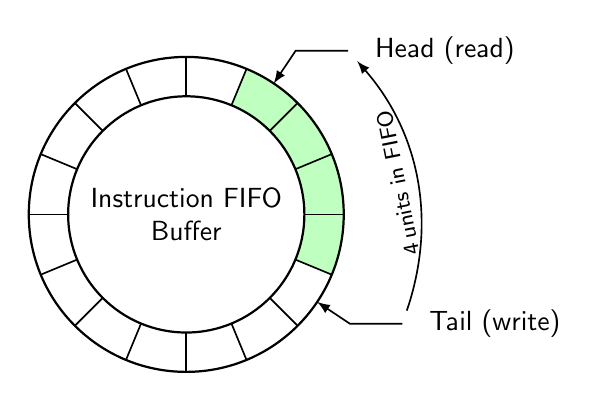
\begin{tikzpicture}[>=latex,font=\sffamily,semithick,scale=2]
        \fill [green!25] (0,0) -- (67.5:1) arc [end angle=-22.5, start angle=67.5, radius=1] -- cycle;
        \draw [thick] (0,0) circle (1);
        \foreach \angle in {90,67.5,...,-67.5}
            \draw (\angle:1) -- (\angle-180:1);
        \node [circle,thick,fill=white,draw=black,align=center,minimum size=3cm] at (0,0) {Instruction FIFO \\ Buffer};
        \draw [<-] (56.25:1) -- (56.25:1.25) -- +(.333,0)
            node [right,inner xsep=.333cm] (Head) {Head (read)};
        \draw [<-] (-33.75:1) -- (-33.75:1.25) -- +(.333,0)
            node [right,inner xsep=.333cm] (Tail) {Tail (write)};
        \draw [->,shorten >=5pt,shorten <=5pt] (Tail.west) to [bend right] 
            node [midway,sloped,above,allow upside down] {\footnotesize 4\,units in FIFO}
        (Head.west);
    \end{tikzpicture}
    \caption{指令 FIFO 原理图}
    \label{fig:InstructionFIFOMechanism}
\end{figure}

\newpage

\section{译码阶段}

译码阶段主要负责指令解码,通用寄存器读取,双发射判断等工作。用于处理数据冲突的旁路模块
也在此处运行。

译码阶段全部逻辑均为组合逻辑。

\subsection{指令解码模块}

指令解码模块由两个 .sv 文件构成,分别为 \href{https://github.com/name1e5s/Sirius/blob/master/decoder\_alpha.sv}{\textbf{decoder\_alpha.sv}}
以及 \href{https://github.com/name1e5s/Sirius/blob/master/decoder\_ctrl.sv}{\textbf{decoder\_ctrl.sv}}。

\textbf{decoder\_alpha} 模块负责将完整的指令按照 MIPS 的编码方式切分为不同的字段,以供译码阶段的各个模块使用,
\textbf{decoder\_ctrl} 模块则根据将指令转换为 Sirius 内部的控制信号,并提供给后续的流水级使用。

\subsection{寄存器文件模块}

寄存器模块在解码阶段以及写回阶段均被使用。寄存器文件内部为 32 个 32 
位的寄存器,实现了 4 个读端口以及 2 个写端口。需要注意的是,在 MIPS32r1 规范中要求
\$0 寄存器读出的数必须为 0,但是我们没有在寄存器文件内实现这一机制,我们把
处理这一要求的逻辑放置在了后续的旁路模块内。

寄存器文件的读端口为组合逻辑,可以在单周期内返回需要的数据;写端口部分为时序逻辑,
写的数据会在下一周期存放到寄存器内。当对一个寄存器号同时进行读写操作时,读出的为
要写入的值。

\subsection{旁路模块}

在译码阶段我们最多可能需要读四个通用寄存器的数值,因此我们需要实例化四个
旁路模块,全部旁路模块使用的都是同一套代码,代码位于 \href{https://github.com/name1e5s/Sirius/blob/master/forwardin\_unit.sv}{\textbf{forwardin\_unit.sv}},
其接口定义见表~\ref{tab:ForwardingUnitInterface}~。

因为引入了双发射技术,对于主流水线和辅助流水线之间的前推的优先级显得尤为重要,我们实现
的旁路模块的各个阶段的优先级如图~\ref{fig:ForwardingUnitPriority}~。旁路模块会
按照优先级顺序确定各个阶段是否有写寄存器文件的请求以及写寄存器号是否与读的寄存器
号相同,如果相同则将该阶段的结果直接作为寄存器读的结果送入下一流水级。如果各个各个流水级
都无需前推,则直接将从寄存器文件内读出的值送入下一流水级。

需要注意的是,如同上一节所叙,我们将处理读取 \$0 寄存器的逻辑放在了这一模块内。具体的
做法是:当判断当前读的寄存器号为 \$0 时,直接返回 0,不做任何前推处理。

\begin{figure}[htpb]
    \centering
    \includegraphics[width=.8\textwidth]{figures/ForwardPriority}
    \caption{前推模块的优先级}
    \label{fig:ForwardingUnitPriority}
\end{figure}

\begin{table}
    \renewcommand\arraystretch{1.25}
    \centering
    \begin{tabular}{lccm{.52\textwidth}}
        \toprule 
        \rowcolor{black!20} \textbf{Signal Name} & \textbf{Width} & \textbf{Direction} & \textbf{Description} \\
        \midrule
        slave\_ex\_reg\_en & 1 & Input & 寄存器使能,当前位于辅流水线执行阶段的指令需要
        写寄存器时,该信号置为 1 \\
        slave\_ex\_addr & 4...0 & Input & 当前位于辅流水线执行阶段的指令需要
        写的寄存器号 \\
        slave\_ex\_data & 31...0 & Input & 当前位于辅流水线执行阶段的结果 \\
        \\
        master\_ex\_reg\_en & 1 & Input & 寄存器使能,当前位于主流水线执行阶段的指令需要
        写寄存器时,该信号置为 1 \\
        master\_ex\_addr & 4...0 & Input & 当前位于主流水线执行阶段的指令需要
        写的寄存器号 \\
        master\_ex\_data & 31...0 & Input & 当前位于主流水线执行阶段的结果 \\
        \\
        slave\_mem\_reg\_en & 1 & Input & 寄存器使能,当前位于辅流水线访存阶段的指令需要
        写寄存器时,该信号置为 1 \\
        slave\_mem\_addr & 4...0 & Input & 当前位于辅流水线访存阶段的指令需要
        写的寄存器号 \\
        slave\_mem\_data & 31...0 & Input & 当前位于辅流水线访存阶段的结果 \\
        \\
        master\_mem\_reg\_en & 1 & Input & 寄存器使能,当前位于主流水线访存阶段的指令需要
        写寄存器时,该信号置为 1 \\
        master\_mem\_addr & 4...0 & Input & 当前位于主流水线访存阶段的指令需要
        写的寄存器号 \\
        master\_mem\_data & 31...0 & Input & 当前位于主流水线访存阶段的结果 \\
        \\
        reg\_addr & 4...0 & Input & 解码阶段需要读的寄存器号 \\
        reg\_data & 31...0 & Input & 从寄存器文件中读出的结果 \\
        \\
        result\_data & 31...0 & Output & 前推后的结果 \\
        \bottomrule
    \end{tabular}
    \caption{旁路单元接口定义}
    \label{tab:ForwardingUnitInterface}
\end{table}

\subsection{双发射判断模块}

双发射判断模块(\href{https://github.com/name1e5s/Sirius/blob/master/dual\_engine.sv}{\textbf{dual\_engine.sv}})
的主要作用是用于判断在当前的情况下是否可以进行双发射。该模块的接口定义见表~\ref{tab:DualIssueInterface}~。

在目前,确定辅流水线是否发射仅需要遵循如下 5 条简单的规则:
\begin{enumerate}
    \item 主流水线不发射,辅流水线必定不发射
    \item 指令 FIFO 仅剩一条指令或者无指令,辅流水线必定不发射
    \item 当主辅流水线存在访问 HiLo 寄存器的指令或者特权指令时,辅
    流水线必定不发射
    \item 当辅流水线中的指令辅流水线无法执行时,辅流水线必定不发射
    \item 当主流水线中的指令与辅流水线的指令之间存在写后读(RAW)相关
    时,辅流水线必定不发射
\end{enumerate}

主流水线以及辅流水线是否会发射的信号会被送回到指令 FIFO 内,指令 FIFO
后续会根据这两个信号更新读指针的位置.

\begin{table}
    \renewcommand\arraystretch{1.25}
    \centering
    \begin{tabular}{lccm{.45\textwidth}}
        \toprule 
        \rowcolor{black!20} \textbf{Signal Name} & \textbf{Width} & \textbf{Direction} & \textbf{Description} \\
        \midrule
        id\_priv\_inst\_master & 1 & Input & 主流水线当前在解码的指令是否为特权指令\\
        id\_wb\_reg\_dest\_master & 4...0 & Input & 主流水线当前解码的指令要写的寄存器号\\
        id\_wb\_reg\_en\_master & 1 & Input & 主流水线当前解码的指令的寄存器文件写使能信号\\
        id\_is\_hilo\_accessed\_master & 1 & Input & 主流水线当前解码的指令是否需要使用到 HiLo 寄存器\\
        \\
        id\_opcode\_slave & 5...0 & Input & 辅流水线当前解码指令的 OpCode\\
        id\_rs\_slave & 4...0 & Input & 辅流水线的源寄存器号\\
        id\_rt\_slave & 4...0 & Input & 辅流水线的另一个源寄存器号\\
        id\_mem\_type\_slave & 1...0 & Input & 辅流水线当前解码的是否需要访存\\
        id\_is\_branch\_instr\_slave & 1 & Input & 辅流水线当前解码的是否是分支跳转指令\\
        id\_priv\_inst\_slave & 1 & Input & 辅流水线当前解码的是否是特权指令\\
        id\_is\_hilo\_accessed\_slave & 1 & Input & 辅流水线当前指令是否需要访问 HiLo\\
        \\
        fifo\_empty & 1 & Input & 指令 FIFO 是否为空\\
        fifo\_almost\_empty & 1 & Input & 指令 FIFO 是否仅剩一条指令\\
        \\
        enable\_master & 1 & Input & 主流水线是否在正常执行指令\\
        enable\_slave & 1 & Input & 是否允许辅流水线当前解码的指令发射\\
        \bottomrule
    \end{tabular}
    \caption{双发射判断模块接口定义}
    \label{tab:DualIssueInterface}
\end{table}

\section{执行阶段}

执行阶段负责执行分支指令,完成算术逻辑运算以及(对于访存指令)生成访存地址
等工作。

大多数的简单的算术逻辑运算可以在 1 周期内完成,但是对于比较 DIV、MULT 等
较为复杂的指令,需要 4 \textasciitilde\  34 个周期来完成,此时就会阻塞流水线等待指令执行完毕。
不过好在多周期指令出现的频率极低,因此直接阻塞不会较大地对影响性能。

我们的乘除法均使用 Xilinx\textsuperscript{\textregistered} 提供的 IP
核实现,其中乘法使用 FPGA 内置的 DSP Slice 实现,4 个周期即可返回结果。除法
则需要 34 个周期。

\subsection{分支单元}

分支单元(\href{https://github.com/name1e5s/Sirius/blob/master/branch.sv}{\textbf{branch.sv}})
用于处理分支指令。其接口见表~\ref{tab:BranchUnitInterface}~。如果该模块发现
当前的指令为分支指令的话,就会根据指令的类型来判断是否进行跳转,其输出信号会被回送
到 PC 以及指令 FIFO 中。

\begin{table}
    \renewcommand\arraystretch{1.25}
    \centering
    \begin{tabular}{lccm{.55\textwidth}}
        \toprule 
        \rowcolor{black!20} \textbf{Signal Name} & \textbf{Width} & \textbf{Direction} & \textbf{Description} \\
        \midrule
        en & 1 & Input & 使能信号 \\
        \\
        pc\_address & 31...0 & Input & 当前执行的指令的 PC 地址 \\
        instruction & 31...0 & Input & 当前执行指令 \\
        is\_branch\_instr & 1 & Input & 该指令是否为跳转分支类指令 \\
        branch\_type & 2...0 & Input & 跳转类型 \\
        \\
        data\_rs & 31...0 & Input & RS 寄存器内的值 \\
        data\_rt & 31...0 & Input & RT 寄存器内的值 \\
        \\
        branch\_taken & 1 & Output & 是否跳转 \\
        branch\_address & 31...0 & Output & 跳转目的地址 \\
        \bottomrule
    \end{tabular}
    \caption{分支单元接口定义}
    \label{tab:BranchUnitInterface}
\end{table}

\subsection{ALU}

ALU 是整个执行阶段,乃至整个 CPU 中最重要的模块之一。Sirius 内置了两个
ALU,分别用于主辅流水线。在这里我们主要介绍在主流水线上使用的 ALU,即 ALU $\alpha$,
用于辅流水线上的 ALU $\beta$ 为 ALU $\alpha$ 取出乘除法以及特权指令后得来的。
不再详细介绍。

ALU $\alpha$ 的代码位于 \href{https://github.com/name1e5s/Sirius/blob/master/alu\_alpha.sv}{\textbf{alu\_alpha.sv}},
其接口定义见表~\ref{tab:ALUAlphaInterface}~。

对于大多数比较简单的算术逻辑指令,我们直接通过调用 SystemVerilog 内置的
运算符号即可完成,但是对于乘、除法这种操作而言,直接调用运算符进行计算必然
会导致执行周期的周期过长,无法有效地提升主频。因此我们在这里使用 Xilinx\textsuperscript{\textregistered}
提供的 IP 核调用对应的片上资源进行运算,并辅以计数器以及运算前/后的求补器完成
各种有符号/无符号乘法运算。

当 ALU 执行过程中出现异常时,对应的 ``exp\_*'' 信号会被置为 1,并随着流水线
进入到下一层级,并在下一层级统一处理。

\begin{table}
    \renewcommand\arraystretch{1.25}
    \centering
    \begin{tabular}{lccm{.55\textwidth}}
        \toprule 
        \rowcolor{black!20} \textbf{Signal Name} & \textbf{Width} & \textbf{Direction} & \textbf{Description} \\
        \midrule
        clk & 1 & Input & 时钟信号\\
        rst & 1 & Input & 复位信号\\
        flush\_i & 1 &Input & 流水线刷新信号\\
        \\
        alu\_op & 5...0 & Input & ALU 操作码\\
        src\_a & 31...0 & Input & 源操作数 1\\
        src\_b & 31...0 & Input & 源操作数 2\\
        src\_hilo & 63...0 & Input & HiLo 寄存器的值\\
        \\
        rd & 4...0 & Input & rd 地址\\
        sel & 2...0 & Input & sel 内容\\
        cop0\_addr & 7...0 & Output & 如果该指令为 MFC0,该
        信号指示从 CP0 中读取什么结果\\
        cop0\_data & 31...0 & Input & 从 CP0 中读到的结果\\
        cop0\_wen & 1 & Output & CP0 写使能\\
        exp\_overflow & 1 & Output & 是否发生了溢出异常\\
        exp\_eret & 1 & Output & 是否正在执行 ERET 指令\\
        exp\_syscal & 1 & Output & 是否正在执行 ERET 指令\\
        exp\_break & 1 & Output & 是否正在执行 break 指令\\
        \\
        hilo\_wen & 1 & Output & HiLo 寄存器写使能\\
        hilo\_result & 63...0 & Output & HiLo 寄存器输出结果\\
        result & 31...0 & Output & 运算结果\\
        stall\_o & 1 & Output & 流水线是否需要暂停\\
        \bottomrule
    \end{tabular}
    \caption{ALU $\alpha$ 接口定义}
    \label{tab:ALUAlphaInterface}
\end{table}

\subsection{HiLo 寄存器}

HiLo 寄存器对外表现为一对寄存器,即 Hi、Lo 两个 32 位的寄存器。在我们的
实现内,Hi、Lo 寄存器被作为一个整体实现,即实现为一个 64 位的寄存器。Hi 寄存器
为这一寄存器的高 32 位,Lo 寄存器为该寄存器的低 32 位的寄存器。

HiLo 寄存器内也实现了一个规模较小的旁路机制,即访存阶段以及写回阶段还未写入到
寄存器内部的数值也可以被前推到执行阶段需要访问 HiLo 寄存器时候获得。

\section{访存阶段}

访存阶段主要负责访问存储器、处理异常。

访存阶段在获取执行阶段送来的访存信号以及地址信息后,根据这些信息向访存单元发出对应
的请求。因为内存访问通常是按字对齐的,但是 MIPS 除了支持 LW、SW 等直接
操作整个字的指令外,还需要支持 LH、SH、LB、SB 等操作半字乃至字节的指令
甚至是一直作为 MIPS 特色的 LWL、SWL 等非对其访问指令。为了支持这些指令,
访存单元在获取所需信号后会将操作转换为 (操作类型,字节使能,操作地址,写数据(如果有)) 的
一个四元组,并发送到访存单元中,访存单元再根据情况决定是对 Data Cache 进行
操作还是动用 AXI 总线访问外部设备。

在进行实际的访存指令之前,异常模块会先行检查是否存在异常,如果存在异常则
取消当前的指令并把对应的 PC 值按照 MIPS 的规范放入 CP0 的 EPC 寄存器内,
同时设置好处理异常所需的各个 CP0 寄存器。中断作为特殊的异常也会在此被处理。

辅流水线在访存阶段什么都不做,仅仅是在未发生异常的情况下直接将所需信号
传送到下一流水级等待处理。

\section{写回阶段}

写回阶段是 Sirius 流水线的最后一个阶段,在该阶段进行的主要是向寄存器文件
以及 HiLo 寄存器写入结果。不再赘述。

\chapter{访存单元}

访存单元主要包含两部分:用于虚实地址转换的 MMU 以及用于加速内存访问的 L1 Cache。

\section{MMU}
MIPS 中的虚实地址转换由 MMU 完成。MIPS 的虚拟地址被分为五部分。其中标号为 $kseg0$ 
以及 $kseg1$ 的部分不需要经过 TLB 的映射,只需将前三位清零即可得到对应的物理地址。
其他部分的地址则需要使用 TLB 进行查表转换。TLB 本质上为一块 CAM,对输入的地址
以及 ASID 进行查表,输出对应的表项。TLB 的核心代码位于 \href{https://github.com/name1e5s/Sirius/blob/SiriusG/tlb\_common.sv}{tlb\_common} 
模块中。

\begin{figure}[htpb]
    \centering
    \includegraphics[width=.4\textwidth]{figures/VirtualAddress}
    \caption{MIPS 虚拟内存映射}
    \label{fig:VirtualAddress}
\end{figure}


TLB 为 8 项全相连接结构,每项均包含有效位、脏位、虚拟地址以及物理地址。
转换时虚拟地址与 TLB 中的条目逐条比较,在找到虚拟地址匹配的条目后,
返回其对应的物理地址以及该地址的状态信息,如果信息无效或者未找到对应的表项,
会抛出对应的异常。为了简化设计,我们的 CPU 设计为固定 4K 页大小,
所以虚拟地址的低 12 位直接成为物理地址的低 12 位,而高 20 位进入 TLB 进行查表操作。
具体转换流程见图~\ref{fig:TLBTran}~。

\begin{figure}[htpb]
    \centering
    \includegraphics[width=.9\textwidth]{figures/TLBTran}
    \caption{地址转换流程}
    \label{fig:TLBTran}
\end{figure}

为了保证性能, TLB 实际上存在 5 个实例,1 个为访存指令服务,其余 4 个
为取指服务。在修改时 5 个实例同步修改,保证 TLB 的一致性。

\newpage

\section{L1 Cache}

设计缓存的目的是为了提高 CPU 的性能。我们的目标是在不影响频率的情况下,
尽可能的设计出容量大、性能高的缓存。我们设计的 L1 Cache 有如下性质:

\begin{enumerate}
    \item 分离的指令缓存与数据缓存
    \item 数据缓存采用写回模式
    \item Index 与 Tag 部分使用物理地址
    \item 单个 Cache 行的大小为 64 字节,以尽可能支持 AXI 总线的猝发传输
    \item 命中读在单周期内返回结果,命中写在一周期后完成
\end{enumerate}

我们实现的指令缓存与数据缓存大小均为 8KB,使用 Xilinx 提供的 Distrubuted 
RAM IP 实现。在缓存中地址的功能分区如下:

\begin{center}
    \begin{bytefield}[endianness=big,bitwidth=1.1em]{32}
        \bitheader{0-31} \\
        \bitbox{19}{Tag} & \bitbox{7}{Index} & 
        \bitbox{4}{Offset} & \bitbox{2}{$\phi$}\\
    \end{bytefield}
\end{center}

\subsection*{状态机}

我们实现的指令缓存是由数据缓存裁剪后并加上双发射相关的代码实现的。因此在这一部分
我们只介绍数据缓存的状态机。

得益于 AXI 读写通道的分离,我们使用了两个状态机分别处理向内存设备的读操作以及写操作,以
尽可能的提升性能。其状态转移简图见~\ref{fig:DCacheRead}~以及~\ref{fig:DCacheWrite}~。

\begin{figure}[htpb]
    \centering
    \includegraphics[width=.6\textwidth]{figures/DCacheRead}
    \caption{数据缓存读状态机}
    \label{fig:DCacheRead}
\end{figure}

\begin{figure}[htpb]
    \centering
    \includegraphics[width=.6\textwidth]{figures/DCacheWrite}
    \caption{数据缓存写状态机}
    \label{fig:DCacheWrite}
\end{figure}


\section{写缓冲}

写缓冲用于加速向内存的写操作。进行性能测试时抓取运行数据可以发现,
由 printf 函数造成的向内存的写操作占据了绝大多数的访存时间,因此我们引入
写缓冲来减少访存造成的流水线暂停次数。

写缓冲被实现为一个 16 项的 FIFO,保存有写入的地址、数据、字节使能等信息。
任何写操作都会暂存在该 FIFO 内。在 FIFO 未满时向内存的
写操作不会导致流水线暂停。当 FIFO 不为空时,访存单元会逐个处理还未完成的写
操作。

为了保证数据的一致性,任何对内存的读操作都会在写缓冲为空后才会执行。

\chapter{系统软件}

\section{SoC 介绍}
为了验证 Sirius CPU 的设计,同时实现启动操作系统更好地完成演示,我们基于大赛提供的 \textbf{soc\_up} 环境
搭建了具有如下特性的 SoC:
\begin{enumerate}
    \item Sirius 双发射 CPU,8KB 指令 Cache, 8KB 数据 Cache
    \item 支持板载 DDR3 SDRAM 内存
    \item 支持从板载 SPI Flash 启动
    \item 支持板载 NAND Flash
    \item 兼容 16550 串口控制器
    \item 100Mbps 以太网络通信
    \item 可运行 uCore 操作系统
\end{enumerate}

\subsection{地址映射}

SoC 中的地址映射由比赛提供的 \textbf{axi\_mux} 模块以及 \textbf{apb\_mux} 模块
实现,地址映射见表~\ref{tab:SoCAddressMapping}~。

\begin{table}
    \renewcommand\arraystretch{1.25}
    \centering
    \begin{tabular}{cccc}
        \toprule 
        \rowcolor{black!20} \textbf{基址} & \textbf{长度} & \textbf{外设名称} & \textbf{接口类型} \\
        \midrule
        0x00000000 & 128MB & DDR3 SDRAM & 存储空间  \\
        0x1fc00000 & 1MB & SPI Flash &  存储空间    \\
        0x1fd00000 & 64KB & GPIO &  寄存器          \\
        0x1fe40000 & 16KB & UART &  寄存器          \\
        0x1fe78000 & 16KB & NAND Flash &  寄存器    \\
        0x1fe80000 & 64KB & SPI Flash & 寄存器      \\
        0xbff00000 & 64KB & MAC & 寄存器            \\
        \bottomrule
    \end{tabular}
    \caption{SoC 地址映射}
    \label{tab:SoCAddressMapping}
\end{table}

\subsection{中断连接}

外设需要依靠中断机制通知 CPU,从而实现高效的 I/O 操作。
MIPS 支持 8 个中断(编号 0 至 7),0、1 号中断为软件中断,
最后一个保留给 CPU 内部的定时器,实际接到外设上的中断号为 2 至 6。连接关系见
表~\ref{tab:SoCInt}~。

\begin{table}
    \renewcommand\arraystretch{1.25}
    \centering
    \begin{tabular}{cc}
        \toprule 
        \rowcolor{black!20} \textbf{中断号} & \textbf{来源} \\
        \midrule
        2 & 以太网控制器 \\
        3 & UART 控制器 \\
        4 & SPI Flash  \\
        5 & NAND Flash \\
        6 & NAND DMA   \\
        \bottomrule
    \end{tabular}
    \caption{中断连接关系}
    \label{tab:SoCInt}
\end{table}

\section{PMON}

Sirius 使用的 PMON 是在大赛官方提供的 PMON 的基础上进行少许修改后
得到的。主要改进是去除我们没有实现的指令。

\subsection{开发环境}

PMON 主要的开发环境为 GCC 的交叉编译工具集。我们使用的 GCC 为
\href{https://mirrors.tuna.tsinghua.edu.cn/}{清华大学开源镜像站}
上托管的 GCC 4.9。

\subsection{构建方法}

在设置好编译环境后,使用如下指令进行编译:

\begin{lstlisting}[language=bash]
	make cfg all tgt=rom CROSS_COMPILE=mipsel-linux- LANG=C
\end{lstlisting}

之后即可在 zloader 文件夹下找到最终生成的 \texttt{gzrom.bin} 文件。
将之烧录到实验箱上的 SPI Flash 内即可启动。

\section{ucore}

Sirius 上的 ucore 是在大赛提供的源码上进行少许修改后得到的,主要的修改为
修正留存的 BUG 以及使代码更加符合我们的硬件实际情况。主要修改如下:

\begin{enumerate}
    \item 在判断中断源时增加对 Status.IM 段的判断
    \item 设置 TLB 的项数为 8
    \item 将 \textbf{KMEMSIZE} 设置为内存的实际大小
\end{enumerate}

\subsection{构建方法}

直接 \texttt{make} 即可。构建后得到 \texttt{ucore-kernel-initrd} 文件。
将之通过串口或者网络加载进 PMON 即可启动 ucore。

\begin{figure}[htpb]
    \centering
    \includegraphics[width=.6\textwidth]{figures/ucore}
    \caption{ucore 运行截图}
    \label{fig:ucore}
\end{figure}

\appendix

\chapter{}
\section{Sirius 指令集} \label{section:ISA}

表~\ref{long}~列出 Sirius 中支持的全部指令,其中浅绿色的为与大赛要求实现的指令相比
Sirius 新增的指令。指令描述来自\cite{MIPS2A}。

\begin{longtable}[c]{| c | l |}
    \caption{Sirius 指令集\label{long}}\\
    
    \hline
    Mnemonic & Description\\
    \hline
    \endfirsthead
    
    \hline
    \multicolumn{2}{|c|}{续表 \ref{long}}\\
    \hline
    Mnemonic  & Description\\
    \hline
    \endhead
    
    \hline
    \endfoot
    
    \hline
    \hline
    \endlastfoot
    
    ADD & Add Word \\
    ADDI & Add Immediate Word \\
    ADDIU & Add Immetiade Add Immediate Unsigned Word \\
    ADDU & Add Unsigned Word \\
    AND & And \\
    ANDI & And Immediate \\
    B & Unconditional Branch \\
    BAL & Branch and Link \\
    BEQ & Branch on Equal \\
    BGEZ & Branch on Greater Than or Equal to Zero \\
    BGEZAL & Branch on Greater Than or Equal to Zero and Link \\
    BGTZ & Branch on Greater Than Zero \\
    BLEZ & Branch on Less Than or Equal to Zero \\
    BLTZ & Branch on Less Than Zero \\
    BLTZAL & Branch on Less Than Zero and Link \\
    BNE & Branch on Not Equal \\
    BREAK & Breakpoint \\
    \rowcolor{green!20} CACHE & Perform Cache Operation \\
    \rowcolor{green!20} CLO & Count Leading Ones in Word \\
    \rowcolor{green!20} CLZ & Count Leading Zeros in Word \\
    DIV & Divide Word \\
    DIVU & Divide Unsigned Word \\
    ERET & Exception Return \\
    J & Jump \\
    JAL & Jump and Link \\
    JALR & Jump and Link Register \\
    JR & Jump Register \\
    LB & Load Byte \\
    LBU & Load Byte Unsigned \\
    LH & Load Halfword \\
    LHU & Load Halfword Unsigned \\
    LUI & Load Upper Immediate \\
    LW & Load Word \\
    \rowcolor{green!20} LWL & Load Word Left \\
    \rowcolor{green!20} LWR & Load Word Right \\
    \rowcolor{green!20} MADD & Multiply and Add Word to Hi,Lo \\
    \rowcolor{green!20} MADDU & Multiply and Add Unsigned Word to Hi,Lo \\
    MFC0 & Move from Coprocessor 0 \\
    MFHI & Move From HI Register \\
    MFLO & Move From LO Register \\
    \rowcolor{green!20} MOVN & Move Conditional on Not Zero \\
    \rowcolor{green!20} MOVZ & Move Conditional on Zero \\
    \rowcolor{green!20} MSUB & Multiply and Subtract Word to Hi,Lo \\
    \rowcolor{green!20} MSUBU & Multiply and Subtract Word to Hi,Lo \\
    MTC0 & Move to Coprocessor 0 \\
    MTHI & Move to HI Register \\
    MTLO & Move to LO Register \\
    \rowcolor{green!20} MUL & Multiply Word to GPR \\
    MULT & Multiply Word \\
    MULTU & Multiply Unsigned Word \\
    NOP & No Operation(Assembly Idiom) \\
    NOR & Not Or \\
    OR & Or \\
    ORI & Or Immediate \\
    SB & Store Byte \\
    SH & Store Halfword \\
    SLL & Shift Word Left Logical \\
    SLLV & Shift Word Left Logical Variable \\
    SLT & Set on Less Than \\
    SLTI & Set on Less Than Immediate \\
    SLTIU & Set on Less Than Immediate Unsigned \\
    SLTU & Set on Less Than Unsigned \\
    SRA & Shift Word Right Arithmetic \\
    SRAV & Shift Word Right Arithmetic Variable \\
    SRL & Shift Word Right Logical \\
    SRLV & Shift Word Right Logical Variable \\
    SSNOP & Superscalar No Operation(Pseudo instruction) \\
    SUB & Subtract Word \\
    SUBU & Subtract Unsigned Word \\
    SW & Store Word \\
    \rowcolor{green!20} SWL & Store Word Left \\
    \rowcolor{green!20} SWR & Store Word Right \\
    \rowcolor{green!20} SYNC & Synchronize Shared Memory \\
    SYSCALL & System Call \\
    \rowcolor{green!20} TLBP & Probe TLB for Matching Entry \\
    \rowcolor{green!20} TLBR & Read Indexed TLB Entry \\
    \rowcolor{green!20} TLBWI & Write Indexed TLB Entry \\
    \rowcolor{green!20} TLBWR & Write Random TLB Entry \\
    \rowcolor{green!20} WAIT & Enter Standby Mode \\
    XOR & Exclusive OR \\
    XORI & Exclusive OR Immediate \\
    \end{longtable}

\section{CP0 寄存器列表} \label{section:CP0}

表~\ref{tab:SiriusCP0}~列出 Sirius 处理器支持的全部 CP0 寄存器列表,其中浅绿色的为与大赛要求实现的寄存器相比
 Sirius 新增的寄存器。寄存器描述来自\cite{MIPS3}。

 \begin{table}
    \renewcommand\arraystretch{1.25}
    \centering
    \begin{tabular}{cclm{.55\textwidth}}
        \toprule 
        \rowcolor{black!20} \textbf{Register Number} & \textbf{Select} & \textbf{Name} & \textbf{Function} \\
        \midrule
        \rowcolor{green!20} 0 & 0 & Index & Index into the TLB array \\
        \rowcolor{green!20} 1 & 0 & Random & Randomly generated index into the TLB array \\
        \rowcolor{green!20} 2 & 0 & EntryLo0 & Low-order portion of the TLB entry for
        even-numbered virtual pages \\
        \rowcolor{green!20} 3 & 0 & EntryLo1 & Low-order portion of the TLB entry for
        odd-numbered virtual pages \\
        \rowcolor{green!20} 4 & 0 & Context & Pointer to page table entry in memory \\
        \rowcolor{green!20} 6 & 0 & Wired & Controls the number of fixed (“wired”) TLB
        entries \\
        \rowcolor{cyan!20} 8 & 0 & BadVAddr & Reports the address for the most recent
        address-related exception \\
        \rowcolor{cyan!20} 9 & 0 & Count & Processor cycle count \\
        \rowcolor{green!20} 10 & 0 & EntryHi & High-order portion of the TLB entry \\
        \rowcolor{cyan!20} 11 & 0 & Compare & Timer interrupt control \\
        \rowcolor{cyan!20} 12 & 0 & Status &  Processor status and control \\
        \rowcolor{cyan!20} 13 & 0 & Cause & Cause of last general exception \\
        \rowcolor{cyan!20} 14 & 0 & EPC & Program counter at last exception \\
        \rowcolor{green!20} 15 & 0 & PRId & Processor identification and revision \\
        \rowcolor{green!20} 16 & 0 & Config &  Configuration register \\
        \rowcolor{green!20} 16 & 1 & Config1 & Configuration register 1 \\

        \bottomrule
    \end{tabular}
    \caption{CP0 寄存器列表}
    \label{tab:SiriusCP0}
\end{table}

\bibliography{DesignReportRef}


\end{document}